\part{The future of PCG}
\frame{\partpage}

\begin{frame}
``You are playing an ``open world'' game, something like Grand Theft Auto or Skyrim.
Instead of going straight to the next mission objective in the city you are in,
you decide to drive (or ride) five hours in some randomly chosen direction.
The game makes up the landscape as you go along, and you end up in a new city that no human player has visited before.
In this city, you can enter any house (though you might have to pick a few locks), talk to everyone you meet,
and involve yourself in a completely new set of intrigues and carry out new missions.
If you would have gone in a different direction, you would have reached a different city
with different architecture, different people and different missions.
Or a huge forest with realistic animals and eremites, or a secret research lab, or whatever the game engine comes up with.''

--- Julian Togelius

{\tiny\url{http://togelius.blogspot.co.uk/2015/10/what-if-videogames-had-actual-ai.html}}
\end{frame}

\begin{frame}{Whole game generation}
	\begin{columns}
		\begin{column}{0.4\textwidth}
			\pause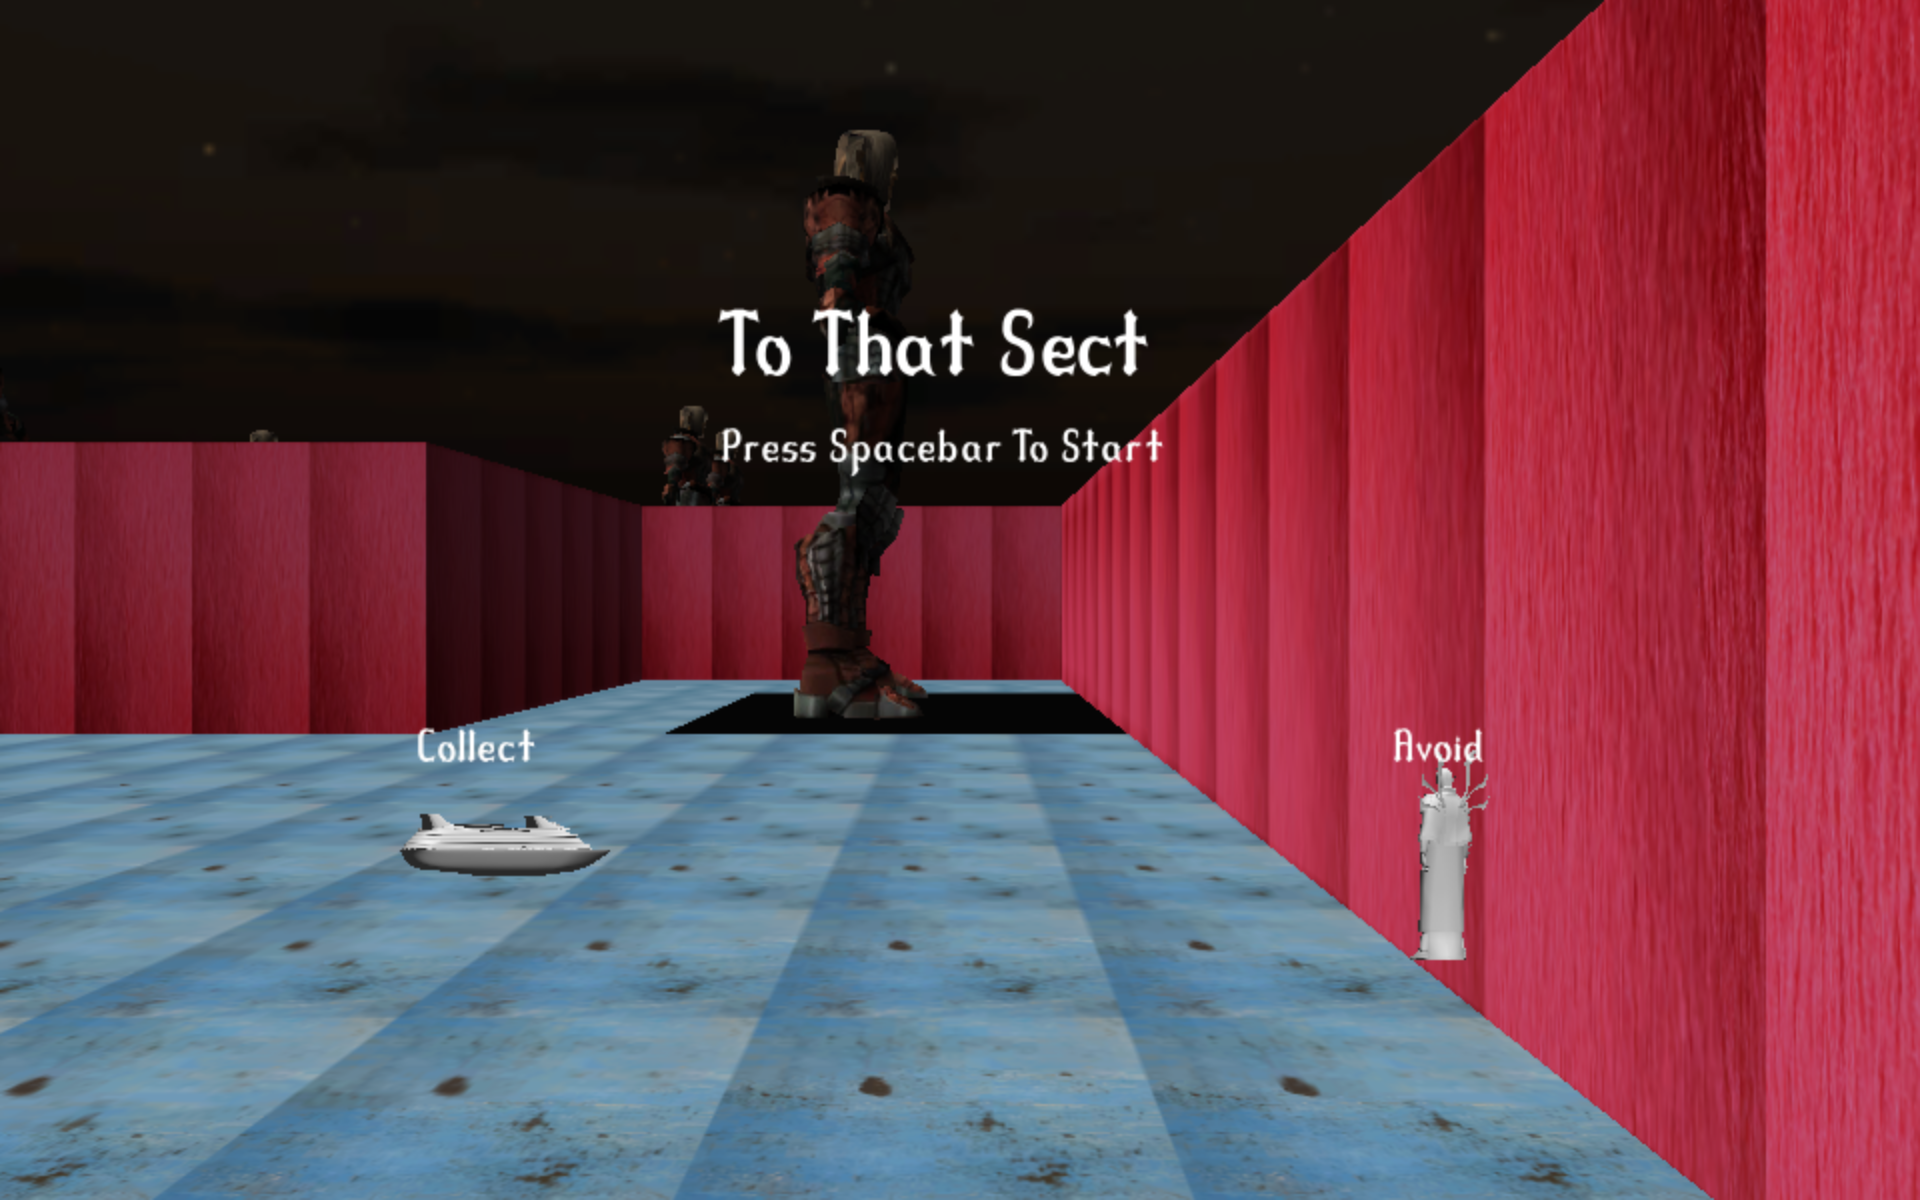
\includegraphics[width=\textwidth]{tothatsect}
		\end{column}
		\begin{column}{0.55\textwidth}
			\begin{itemize}
				\pause\item E.g.\ ANGELINA (Michael Cook)
				\pause\item Generate \textbf{entire games} from scratch, possibly using ideas or themes provided by the user
				\pause\item \textbf{Democratise} game design --- create games in \textbf{collaboration} with a
					non-skilled user
					\begin{itemize}
						\pause\item (i.e.\ make it so that you don't need to do a degree to learn how to make games...)
					\end{itemize}
			\end{itemize}
		\end{column}
	\end{columns}
\end{frame}

\begin{frame}{Computational creativity}
	\begin{columns}
		\begin{column}{0.4\textwidth}
			\pause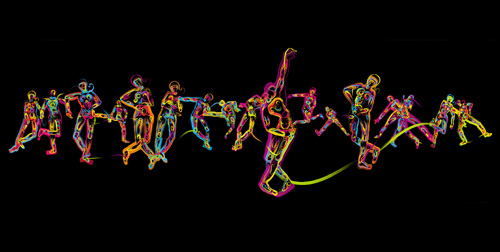
\includegraphics[width=\textwidth]{paintingfool}
			
			\vspace{2ex}
			
			\pause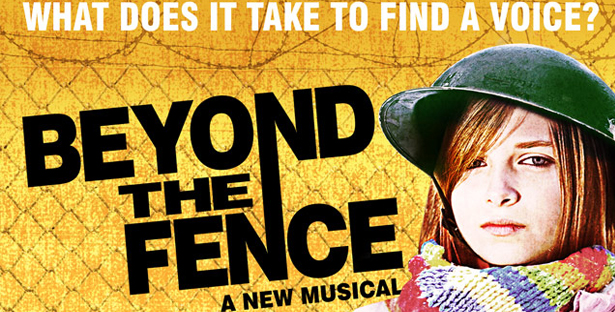
\includegraphics[width=\textwidth]{beyondthefence}
		\end{column}
		\begin{column}{0.55\textwidth}
			\begin{itemize}
				\pause\item Open question: can an AI system be \textbf{creative}?
				\pause\item Beyond \textbf{mere generation}
				\pause\item Beyond generating \textbf{content} to generating \textbf{ideas}
			\end{itemize}
		\end{column}
	\end{columns}
\end{frame}
